\documentclass{amsart}

\usepackage[utf8]{inputenc}
\usepackage[T2A]{fontenc}
\usepackage[english,russian]{babel}
\usepackage{amsthm,amsmath,amsfonts,amssymb}
\usepackage{fullpage}
\usepackage{eufrak}
\usepackage{bbm}

%%% Дополнительная работа с математикой
\usepackage{amsfonts,amssymb,amsthm,mathtools} % AMS
\usepackage{amsmath}
\usepackage{icomma}

%% Шрифты
\usepackage{euscript}	% Шрифт Евклид
\usepackage{mathrsfs}	% Красивый матшрифт

%% Свои команды
\DeclareMathOperator{\lb}{\mathop{lb}}	% логарифм по основанию 2
\DeclareMathOperator{\sgn}{\mathop{sgn}}	% сигнум
\renewcommand{\Im}{\mathop{\mathrm{Im}}\nolimits}	% мнимая часть
\renewcommand{\Re}{\mathop{\mathrm{Re}}\nolimits}	% вещественная часть
\renewcommand{\emptyset}{\varnothing}	% пустое множество
\renewcommand{\le}{\leqslant}	% отечественная версия "меньше или равно"
\renewcommand{\ge}{\geqslant}	% отечественная версия "больше или равно"
\renewcommand{\epsilon}{\varepsilon}	% стандартная "эпсилон"
\renewcommand{\phi}{\varphi}	% стандартная "фи"
\newcommand{\const}{\mathrm{const}}	% константа

%% Множества чисел
\DeclareMathOperator{\Natural}{\mathbb{N}}	% Натуральные числа
\DeclareMathOperator{\Integer}{\mathbb{Z}}	% Целые числа
\DeclareMathOperator{\Integerp}{\mathbb{Z}_{+}}	% Целые неотрицательные числа
\DeclareMathOperator{\Rational}{\mathbb{Q}}	% Рациональные числа
\DeclareMathOperator{\Real}{\mathbb{R}}	% Вещественные числа
\DeclareMathOperator{\Realp}{\mathbb{R}_{>0}}	% Вещественные положительные числа
\DeclareMathOperator{\Realn}{\mathbb{R}_{<0}}	% Вещественные отрицательные числа
\DeclareMathOperator{\Realnn}{\mathbb{R}_{\ge 0}}	% Вещественные неотрицательные числа
\DeclareMathOperator{\Realnp}{\mathbb{R}_{\le 0}}	% Вещественные неположительные числа
\DeclareMathOperator{\Complex}{\mathbb{C}}	% Комплексные числа

%% Заглавные греческие буквы
\DeclareMathOperator{\Alpha}{\mathrm{A}}	% Альфа
\DeclareMathOperator{\Beta}{\mathrm{B}}	% Вета
\DeclareMathOperator{\Epsilon}{\mathrm{E}}	% Эпсилон
\DeclareMathOperator{\Zeta}{\mathrm{Z}}	% Дзета
\DeclareMathOperator{\Eta}{\mathrm{H}}	% Эта
\DeclareMathOperator{\Iota}{\mathrm{I}}	% Йота
\DeclareMathOperator{\Kappa}{\mathrm{K}}	% Каппа
\DeclareMathOperator{\Mu}{\mathrm{M}}	% Мю
\DeclareMathOperator{\Nu}{\mathrm{N}}	% Ню
\DeclareMathOperator{\Omicron}{\mathrm{O}}	% Омикрон
\DeclareMathOperator{\Rho}{\mathrm{P}}	% Ро
\DeclareMathOperator{\Tau}{\mathrm{T}}	% Тау
\DeclareMathOperator{\Chi}{\mathrm{X}}	% Хи

%% Теория вероятностей
\renewcommand{\Prob}{\mathbb P}	% вероятность
\newcommand{\Expect}{\mathbb E}	% математическое ожидание
\renewcommand{\Variance}{\mathbb D}	% дисперсия
\newcommand{\Entropy}{\mathbb H}	% энтропия
\DeclareMathOperator{\cov}{\mathop{cov}}	% ковариация
\DeclareMathOperator{\supp}{\mathop{supp}}	% носитель
\DeclareMathOperator{\Skewness}{\mathop{Skew}}	% коэффициент асимметрии
\DeclareMathOperator{\Kurtosis}{\mathop{Kurt}}	% коэффициент эксцесса

%%% Статистический анализ
\newcommand*{\moment}[1]{\overline{#1}}	% выборочный момент
\DeclareMathOperator{\hskew}{\mathop{\widehat{Skew}}}	% выборочный коэффициент асимметрии
\DeclareMathOperator{\hkurt}{\mathop{\widehat{Kurt}}}	% выборочный коэффициент эксцесса
%% Однопараметрические распределения
\newcommand*{\chisq}[1]{\chi^2_{#1}}	% Распределение хи-квадрат
\newcommand*{\Stud}[1]{\mathcal{S}_{#1}}	% Распределение Стьюдента
\newcommand*{\Exp}[1]{\mathop{\mathrm{Exp}}(#1)}	% Показательное распределение
\newcommand*{\Bern}[1]{\mathop{\mathrm{Bern}}(#1)}	% Распределение Бернулли
\newcommand*{\Geom}[1]{\mathop{\mathrm{Geom}}(#1)}	% Геометрическое распределение
\newcommand*{\Pois}[1]{\mathop{\mathrm{Pois}}(#1)}	% Распределение Пуассона
%% Двухпараметрические распределения
\newcommand*{\FS}[2]{\mathcal{F}_{#1, #2}}	% Распределение Фишера-Снедекора
\newcommand*{\Norm}[2]{\mathcal{N}(#1, #2)}	% Нормальное распределение
\newcommand*{\Unif}[2]{\mathcal{U}(#1, #2)}	% Равномерное распределение
\newcommand*{\DE}[2]{\mathop{\mathrm{DE}}(#1, #2)}	% Распределение Лапласа
\newcommand*{\Cauchy}[2]{\mathop{\mathrm{C}}(#1, #2)}	% Распределение Коши
\newcommand*{\Binom}[2]{\mathop{\mathrm{Binom}}(#1, #2)}	% Биномиальное распределение
\newcommand*{\Betadist}[2]{\mathop{\mathrm{Beta}}(#1, #2)}	% Бета-распределение
\newcommand*{\Gammadist}[2]{\mathop{\mathrm{Gamma}}(#1, #2)}	% Гамма-распределение
%% Ажурные и готические буквы
\newcommand*{\Acl}{\mathcal{A}}	% A красивое
\newcommand*{\Ccl}{\mathcal{C}}	% C красивое
\newcommand*{\Fcl}{\mathcal{F}}	% F красивое
\newcommand*{\Icl}{\mathcal{I}}	% I красивое
\newcommand*{\Kcl}{\mathcal{K}}	% K красивое
\newcommand*{\Pcl}{\mathcal{P}}	% P красивое
\newcommand*{\Ycl}{\mathcal{Y}}	% Y красивое
\newcommand*{\Afr}{\mathfrak{A}}	% A готическое
\newcommand*{\Bfr}{\mathfrak{B}}	% B готическое
\newcommand*{\Ffr}{\mathfrak{F}}	% F готическое
\newcommand*{\Kfr}{\mathfrak{K}}	% K готическое
\newcommand*{\Xfr}{\mathfrak{X}}	% X готическое
%% Теория оценивания
\newcommand*{\ind}[1]{\mathbbm{1}_{\lbrace #1 \rbrace}}	% индикаторная функция
\newcommand*{\bias}[2]{\mathop{\mathrm{bias}}\nolimits_{#1}(#2)}	% смещение

%% Перенос знаков в формулах (по Львовскому)
\newcommand*{\hm}[1]{#1\nobreak\discretionary{}
	{\hbox{$\mathsurround=0pt #1$}}{}}

%%% Работа с картинками
\usepackage{graphicx,xcolor}	% Для вставки рисунков
\graphicspath{{images/}{images2/}}	% папки с картинками
\setlength\fboxsep{3pt}	% Отступ рамки \fbox{} от рисунка
\setlength\fboxrule{1pt}	% Толщина линий рамки \fbox{}
\usepackage{wrapfig}	% Обтекание рисунков и таблиц текстом
\RequirePackage{caption}
\DeclareCaptionLabelSeparator{defffis}{ "--- }
\captionsetup{justification=centering,labelsep=defffis}
\usepackage{float}
\usepackage{tikz}
\usepackage{pgfplots}
\pgfplotsset{compat=newest}
\usetikzlibrary{patterns}
\usetikzlibrary{calc}

%%% Работа с таблицами
\usepackage{array,tabularx,tabulary,booktabs}	% Дополнительная работа с таблицами
\usepackage{longtable}	% Длинные таблицы
\usepackage{multirow}	% Слияние строк в таблице
\usepackage{makecell}
\usepackage{multicol}


\renewcommand{\qedsymbol}{}

\newtheorem{problem}{Задание}

\begin{document}
	\newcommand{\problemset}[1]{
		\begin{center}
			\Large #1
		\end{center}
	}

	\begin{tabbing}
	\hspace{11cm} \= Студент: \= Божко-Домбровский Тимофей \\																			
	\> Группа: \> 2375 \\
	\> Вариант: \> 5 \\	
	\> Дата: \> \today
\end{tabbing}
\hrule
\vspace{1cm}	% файл с заголовком
	\problemset{Теория вероятностей и математическая статистика}
\problemset{Индивидуальное домашнее задание №4}

% Команда ниже задает "название" или слово, которое будет
% отображаться вместо proof или "доказательство"
% поскольку у нас в ИДЗ задачи - то нужно слово "Решение"
\renewcommand*{\proofname}{Решение}
Матрица вероятностей перехода однородной цепи Маркова имеет вид
\[
P = \frac{1}{10}\begin{pmatrix}
    2 & 0 & 0 & 0 & 2 & 4 & 2 & 0 \\
    0 & 4 & 0 & 6 & 0 & 0 & 0 & 0 \\
    3 & 0 & 4 & 0 & 2 & 0 & 1 & 0 \\
    0 & 5 & 0 & 5 & 0 & 0 & 0 & 0 \\
    1 & 0 & 4 & 0 & 3 & 2 & 0 & 0 \\
    2 & 0 & 0 & 0 & 2 & 5 & 1 & 0 \\
    4 & 0 & 3 & 0 & 0 & 3 & 0 & 0 \\
    0 & 3 & 0 & 1 & 0 & 3 & 3 & 0 \\
\end{pmatrix}
\]

%%%%%%%%%%%%%% ЗАДАНИЕ №1 %%%%%%%%%%%%%%
%% Условие задания №1
\begin{problem}
Определить матрицу вероятностей перехода за два шага.
\end{problem}

%% Решение задания №1
\begin{proof}
\[
P^{(2)} = P^2 = \frac{1}{100}\begin{pmatrix}
    22 & 0  & 14 & 0  & 18 & 38 & 8  & 0 \\
    0  & 46 & 0  & 54 & 0  & 0  & 0  & 0 \\
    24 & 0  & 27 & 0  & 20 & 19 & 10 & 0 \\
    0  & 45 & 0  & 55 & 0  & 0  & 0  & 0 \\
    21 & 0  & 28 & 0  & 23 & 20 & 8  & 0 \\
    20 & 0  & 11 & 0  & 20 & 40 & 9  & 0 \\
    23 & 0  & 12 & 0  & 20 & 31 & 14 & 0 \\
    18 & 17 & 9  & 23 & 6  & 24 & 3  & 0
\end{pmatrix}
\]
\end{proof}

%%%%%%%%%%%%%% ЗАДАНИЕ №2 %%%%%%%%%%%%%%
%% Условие задания №2
\begin{problem}
Выделить классы сообщающихся состояний.
\end{problem}

%% Решение задания №2
\begin{proof}
Нарисуем граф (рис.1). На рисунке все веса делить на 10.\\
\begin{figure}[h!]
    \centering
    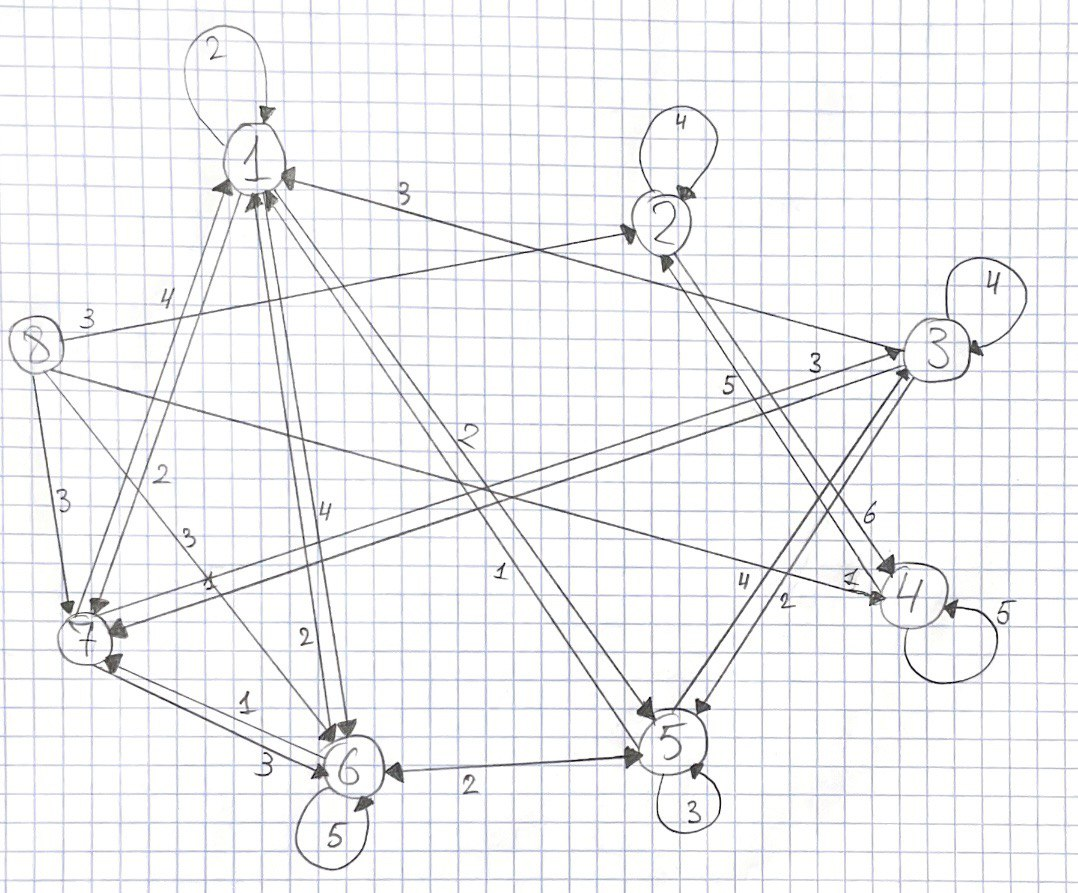
\includegraphics[width=0.5\linewidth]{1.jpeg}
    \caption{}
    \label{fig:enter-label}
\end{figure}
Смотрим, анализируем и получаем следующие классы сообщающихся состояний:\\
$E_0 = $ {8}\\
$E_1 = $ {1, 3, 5, 6, 7}\\
$E_2 = $ {2, 4}\\
\end{proof}

%%%%%%%%%%%%%% ЗАДАНИЕ №3 %%%%%%%%%%%%%%
%% Условие задания №3
\begin{problem}
Есть ли невозвратные состояния?
\end{problem}

%% Решение задания №3
\begin{proof}
Да. Состояние 8. В него невозможно вернуться, покинув его. Это невозвратное (или несущественное) состояние.
\end{proof}

%%%%%%%%%%%%%% ЗАДАНИЕ №4 %%%%%%%%%%%%%%
%% Условие задания №4
\begin{problem}
Найти период в каждом из классов.
\end{problem}

%% Решение задания №4
\begin{proof}
Матрица класса 1:
\[
P_1 = \frac{1}{10}\begin{pmatrix}
    2 & 0 & 2 & 4 & 2 \\
    3 & 4 & 2 & 0 & 1 \\
    1 & 4 & 3 & 2 & 0 \\
    2 & 0 & 2 & 5 & 1 \\
    4 & 3 & 0 & 3 & 0
\end{pmatrix}
\]
m = 1 для i = {1, 3, 5, 6}.\\
\[
P_1^2 = \frac{1}{100}\begin{pmatrix}
    14 & 8  & 18 & 32 & 4 \\
    24 & 27 & 20 & 19 & 4 \\
    21 & 28 & 23 & 20 & 6 \\
    20 & 11 & 20 & 40 & 5 \\
    23 & 12 & 20 & 31 & 6
\end{pmatrix}
\]
m = 2 для i = 7.\\
НОД(1, 2) = 1, то есть период класса 1 равен 1, он апериодичный\\
Матрица класса 2:
\[
P_1 = \frac{1}{10}\begin{pmatrix}
    4 & 6 \\
    5 & 5
\end{pmatrix}
\]
Тут всего один m = 1 для i = {2, 4}, значит что период класса 2 равен 1, он апериодичный.
\end{proof}

%%%%%%%%%%%%%% ЗАДАНИЕ №5 %%%%%%%%%%%%%%
%% Условие задания №5
\begin{problem}
Вычислить финальные вероятности в каждом классе.
\end{problem}

%% Решение задания №5
\begin{proof}
Для класса 1:
\begin{gather*}
    x = (p_1, p_3, p_5, p_6, p_7)\\
    \begin{cases}
        (P_1^T - I)x^T = 0 \\
        \sum_i p_i = 1
    \end{cases} \Rightarrow \\
    \begin{cases}
        (10P_1^T - 10I)x^T = 0 \\
        \sum_i p_i = 1
    \end{cases}
\end{gather*}
В первом уравнении системы получили систему однородных уравнений. Она имеет матрицу:
\[
\begin{pmatrix}
    -8 & 3 & 1 & 2 & 4 \\
    0 & -6 & 4 & 0 & 3 \\
    2 & 2 & -7 & 2 & 0 \\
    4 & 0 & 2 & -5 & 3 \\
    2 & 1 & 0 & 1 & -10 \\
\end{pmatrix}
\]
Решаем систему и получаем ответ $x = (\frac{1229}{524}p_7, \frac{513}{262}p_7, \frac{573}{262}p_7, \frac{439}{131}p_7, p_7)$. Воспользуемся вторым условием $\sum_i p_i = 1$ и получим:\\
\begin{gather*}
    p_1 = \frac{1229}{5681}\approx 0.2163\\
    p_3 = \frac{54}{299}\approx 0.1806\\
    p_5 = \frac{1146}{5681}\approx 0.2017\\
    p_6 = \frac{1756}{5681}\approx 0.3091\\
    p_7 = \frac{524}{5681}\approx 0.0922
\end{gather*}

Для класса 2:
\begin{gather*}
    x = (p_2, p_4)\\
    \begin{cases}
        (P_2^T - I)x^T = 0 \\
        \sum_i p_i = 1
    \end{cases} \Rightarrow \\
    \begin{cases}
        (10P_2^T - 10I)x^T = 0 \\
        \sum_i p_i = 1
    \end{cases}
\end{gather*}
Матрица однордной системы:
\[
\begin{pmatrix}
    -6 & 5 \\
     6 & -5
\end{pmatrix}
\]
Её решение: $x = (\frac{5}{6}p_4, p_4)$. Воспользуемся вторым условием и получим:\\
\begin{gather*}
    p_2 = \frac{5}{11}\approx 0.4545\\
    p_4 = \frac{6}{11}\approx 0.5454\\
\end{gather*}
Поскольку состояние 8 - несущественное, $p_8 = 0$.
\end{proof}

Задания 6 и 7: https://github.com/timohahaa/PT-MS/blob/main/sim.ipynb	% файл с решениями
        %\problemset{Теория вероятностей и математическая статистика}
\problemset{Индивидуальное домашнее задание №0}	% поменяйте номер ИДЗ

\renewcommand*{\proofname}{Решение}

%%%%%%%%%%%%%% ЗАДАНИЕ №1 %%%%%%%%%%%%%%
%% Условие задания №1
\begin{problem}
	Из урны, в которой лежат $ K $ белых и $ L $ чёрных шаров, наудачу выбирают один шар. Чему равна вероятность того, что этот шар "--- белый?
\end{problem}

%% Решение задания №1
\begin{proof}
	Пусть $ A $ "--- событие, что достали белый шар.
	Количество всех исходов будет равно: $ \#\Omega \hm= K + L $.
	
	Тогда количество благоприятных исходов (наступления события $ A $) равно: $ \#A = K $.
	
	Отсюда получаем, что вероятность наступления события $ A $ равна:
	\[ \Prob A = \cfrac{\#A}{\#\Omega} = \cfrac{K}{K + L}. \]
\end{proof}

%%%%%%%%%%%%%% ЗАДАНИЕ №2 %%%%%%%%%%%%%%
%% Условие задания №2
\begin{problem}
	Распределение случайной величины $ \xi $ задано таблицей:
	\begin{center}
		\begin{tabular}{|c|c|c|c|c|c|}
		\hline
		$ \xi $ & 1 & 2 & 4 & 6 & $ \Sigma $ \\
		\hline
		$ \mathbb{P} $ & 0,1 & 0,2 & 0,6 & 0,1 & 1 \\
		\hline
		\end{tabular}
	\end{center}
	Вычислить $ \Expect\xi $, $ \Variance\xi $, $ \Entropy\xi $ (в натах) и распределение $ \eta = \sin(\pi\xi/3) $.
\end{problem}

%% Решение задания №2
\begin{proof}
	Математическое ожидание дискретной случайной величины $ \xi $ задаётся формулой:
	\[ \Expect\xi = \sum_{i \colon p_i > 0}a_ip_i. \]
	Отсюда получаем:
	\[ \Expect\xi = 1 \cdot 0,1 + 2 \cdot 0,2 + 4 \cdot 0,6 + 6 \cdot 0,1 = 3,5. \]
	Дисперсия дискретной случайной величины $ \xi $ задаётся формулой:
	\[ \Variance\xi = \sum_{i \colon p_i > 0}(a_i - \mathbb E\xi)^2p_i. \]
	Отсюда получаем:
	\[ \Variance\xi = (1 - 3,5)^2 \cdot 0,1 + (2 - 3,5)^2 \cdot 0,2 + (4 - 3,5)^2 \cdot 0,6 + (6 - 3,5)^2 \cdot 0,1 = 1,85. \]
	Энтропия дискретной случайной величины $ \xi $ задаётся формулой:
	\[ \Entropy\xi = -\sum_{i \colon p_i > 0}p_i\log_bp_i. \]
	Необходимо вычислить энтропию в натах, т~е. $ b = e $. Получим:
	\[ \Entropy\xi = -(0,1 \cdot \ln0,1 + 0,2 \cdot \ln0,2 + 0,6 \cdot \ln0,6 + 0,1 \cdot \ln0,1) \approx 1,0889. \]
	Носитель случайной величины $ \xi $ имеет вид: $ \supp \xi = \lbrace 1, 2, 4, 6 \rbrace $. Тогда носитель случайной величины $ \eta $ будет иметь вид: $ \supp \eta = \left\lbrace -\frac{\sqrt{3}}{2}, 0, \frac{\sqrt{3}}{2} \right\rbrace  $. Найдём вероятности появления каждого числа:
	\begin{align*}
		\Prob(\eta = -\sqrt{3}/2) &= \Prob(\xi = 4) = 0,6. \\
		\Prob(\eta = 0) &= \Prob(\xi = 6) = 0,1. \\
		\Prob(\eta = \sqrt{3}/2) &= \Prob(\xi = 1) + \Prob(\xi = 2) = 0,3.
	\end{align*}
	Таким образом, можно записать распределение случайной величины $ \eta $ в виде таблицы:
	\begin{center}
		\begin{tabular}{|c|c|c|c|c|}
			\hline
			$ \eta $  & $ -\sqrt{3}/2 $ & 0   & $ \sqrt{3}/2 $ & $ \Sigma $ \\ \hline
			$ \Prob $ & 0,6             & 0,1 & 0,3            & 1          \\ \hline
		\end{tabular}
	\end{center}
\end{proof}

%%%%%%%%%%%%%% ЗАДАНИЕ №3 %%%%%%%%%%%%%%
%% Условие задания №3
\begin{problem}
	Условие задачи №3.
\end{problem}

%% Решение задания №3
\begin{proof}
	Решение задачи №3.
\end{proof}
\end{document}